\documentclass{article}
\usepackage[margin=1in]{geometry}
\usepackage[utf8]{inputenc}
\usepackage[english]{babel}
\usepackage{amssymb}
\usepackage{amsmath}
\usepackage{graphicx}
\setlength{\parindent}{4em}
\setlength{\parskip}{1em}
\usepackage{ragged2e}
\usepackage{blindtext}
\usepackage{setspace}
\renewcommand{\baselinestretch}{1.0}

\title{%
   \Large{Úloha 1 - Geometrické vyhledávání bodu} \\
  \large{Algoritmy počítačové kartografie}}
\author{Tomáš Hřebec, Kateřina Obrazová}
\date{Praha 2022}

\begin{document}
\onehalfspacing
\maketitle
\justifying
\section{\large{Zadání úlohy}}
\subsection{\small{Povinná část}}
\textit{Vstup: Souvislá polygonová mapa n polygonů $\{P_{1}, ..., P_{n}\}$,~analyzovaný~bod~q.}
\vspace{0.2cm}\\
\textit{Výstup: $P_{i}$, $q\in P_{i}$.}
\vspace{0.2cm}\\
Nad polygonovou mapou implementujete Winding Number Algorithm pro geometrické vyhledání incidujícího polygonu obsahující zadaný bod \emph{q}.
\vspace{0.2cm}\\
Nalezený polygon graficky zvýrazněte vhodným způsobem (např.~vyplněním, šrafováním, blikáním). Grafické rozhraní vytvořte s využitím frameworku QT.
\vspace{0.2cm}\\
Pro generování nekonvexních polygonů můžete navrhnout vlastní algoritmus či použít existující geografická data (např. mapa evropských států). 
\vspace{0.2cm}\\
Polygony budou načítány z textového souboru ve Vámi zvoleném formátu. Pro datovou reprezentaci jednotlivých polygonů použijte špagetový model.
\subsection{\small{Volitelná část}}
Analýza polohy bodu (uvnitř/vně) metodou Ray Algorithm.
\vspace{0.2cm}\\
Ošetření singulárního případu u Ray Algorithm: bod leží na hraně polygonu. \vspace{0.2cm}\\
Ošetření singulárního případu u obou algoritmů: bod je totožný s vrcholem jednoho či více polygonů.
\vspace{0.2cm}\\
Zvýraznění všech polygonů pro oba výše uvedené singulární případy.
\clearpage
\newpage
\section{\large{Popis problému}}
Je dán fixní polygon \emph{P} s \emph{n} počtem stran a bod \emph{q}. Leží bod \emph{q} v polygonu \emph{P}? Tento dotaz můžeme přirovnat ke kliknutí myši na obrazovku počítače. Avšak hardware stroje může umožnit řešení, která se vyhýbají geometrii. V našem případě uvažujeme problém z hlediska výpočetní geometrie. (O'Rourke 1998) 
\subsection{\small{Poloha bodu vůči mnohoúhelníku (polygonu)}}
Používají se dva přístupy, kdy je možné otestovat, zda bod \emph{q} je vnitřním bodem rovinného polygonu.
\subsubsection{Konvexní polygon}
Konvexní polygon vzniká jako průnik polorovin definovaných shodně nalevo (napravo) od jeho orientovaných hran. \textit{„Zvolíme-li shodnou orientaci vlevo, pak vnitřní bod musí pro všechny hrany ležet v levých  polorovinách vymezených hranami. (Obr. 1) Použijeme test velikosti orientovaného obsahu trojúhelníka $P_{i}P_{i+1}$q, který musí být pro všechny vrcholy $P_{i}$ vždy $<=$ 0." (Žára a kol. 2004, str. 564)} 
\[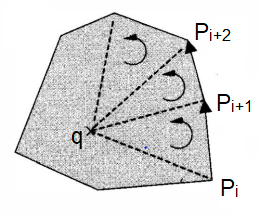
\includegraphics[height=35mm]{images/q_konvexni.PNG}\]
\[\textit{\footnotesize{Obr. 1 - Zjišťování polohy bodu vůči konvexnímu polygonu}}\\\]
\subsubsection{Nekonvexní polygon}
Z testovaného bodu \emph{q} libovolným směrem vyšleme polopřímku a počítáme, kolikrát protne hranici mnohoúhelníku. (Obr. 2) Je-li počet protnutí lichý, bod \emph{q} je uvnitř mnohoúhelníku (polygonu). Je-li počet protnutí sudý, bod \emph{q} leží vně mnohoúhelníku (polygon). (Žára a kol. 2004)
\[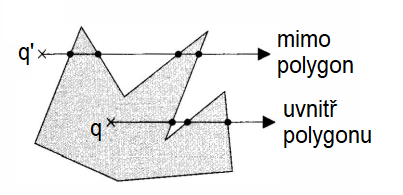
\includegraphics[height=35mm]{images/q_nekonvexni.PNG}\]
\[\textit{\footnotesize{Obr. 2 - Zjišťování polohy bodu vůči nekonvexnímu polygonu}}\\\]
\clearpage
\newpage
\section{\large{Popis algoritmu}}
Pro řešení konvexního polygonu se používá opakovaný Half-Plane Test a Ray Crossing algoritmus. Pro řešení nekonvexního polygonu se používájí algoritmy Winding Number a Ray Crossing generalizovaný pro nekonvexní polygony.
\subsection{\small{Ray Crossing Method}}
Algoritmus vede z bodu \emph{q}polopřímku (paprsek, ray) \emph{R} v libovolném směru. Dále je zjištěn počet průsečíků \emph{R} s $\partial$\emph{P}. Je-li počet prolnutí lichý, bod $q \in P$, pokud sudý, bod $q \notin P$. (Obr. 3)
\[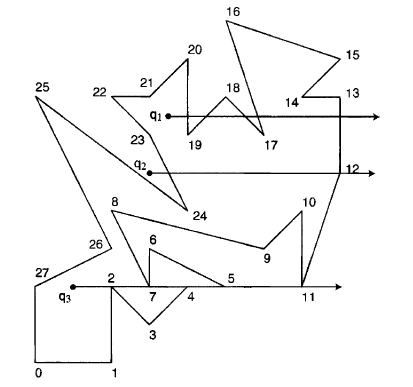
\includegraphics[height=60mm]{images/ray_crossing.PNG}\]
\[\textit{\footnotesize{Obr. 3 - Ray Crossing Algoritmus}}\\\]
Ke zjištění polohy bodu $q_{3}$, je potřeba upravit paprsek \emph{R} tak, aby byl horizontálně doprava. \textit{„Jedním ze způsobů, jak odstranit většinu obtíží, je vyžadovat, aby se hrana mohla počítat jako křížení R, jeden z koncových bodů e musí být přísně nad R a druhý koncový bod na nebo pod. Neformálně se má za to, že e zahrnuje svůj spodní koncový bod, ale vylučuje svůj horní koncový bod. Při použití této konvence pro q3 (Obr. 3) se hrany (1, 2) a (2, 3) nekříží (žádná hrana nemá koncový bod striktně výše). Hrany (6, 7) a (7,8) se počítají jako křížení ($v_{7}$ je na nebo pod), (3,4) a (4,5) se nekříží a (5, 6), (10, 11 ), a (11, 12) se všechny kříží. Celkový počet pěti křížení znamená, že $q\in P$. Všimněte si, že žádná hrana kolineární s paprskem se nepočítá jako křížení, protože nemá žádný bod přísně nahoře" (O'Rourke 1998, s. 240)."}\\
V rámci tohoto algoritmu mohou nastat situace, které je nutné v rámci algoritmu ošetřit:\begin{itemize}
    \item bod $q$ je totožný s vrcholem,
    \item polopřímka $R$ je kolineární s hranou tj. ležící na stejné přímce.
\end{itemize}
Ovšem tato varianta algoritmu neumí detekovat stav $q \in \partial P$. Je tedy nutné použít dva paprsky s opačnou orientací $r_{1}$ (levostranný), $r_{2}$ (pravostranný), jejichž počet průsečíků $k_{l}$ a $k{r}$ je udržován. Pokud tedy $q \in \partial P$, tak počet levostranných a pravostranných průsečíků je různý. 
\vspace{0.2cm}\\
Hlubší popis algoritmu je v následujícím pseudokódu:\\
\vspace{0.2cm}\\
\indent\textit{\textrm{1.~}Inicializuj počet průsečíků v pravé polorovině na 0}\\
\indent\textit{\textrm{2.~}Inicializuj počet průsečíků v levé polorovině na 0}\\
\indent\textit{\textrm{3.~}Zjisti počet vrcholů polygonu $n$}\\
\indent\textit{\textrm{4.~}\textbf{Projdi} jednotlivé vrcholy $p_{i}$ polygonu:}\\
\indent\indent\textit{\textrm{5.~}Souřadnice vrcholů $p_{i}$ a $p_{i-1}$ transformuj do lokálního systému s počátkem v $q$}\\
\indent\indent\textit{\textrm{6.~}\textbf{Když} bod $p_{i}$ leží v počátku:}\\
\indent\indent\indent\textit{\textrm{7.~}Vrchol $p_{i}$ je totožný s $q$ a vrať, že $q$ je uvnitř polygonu a ukonči výpočet}\\
\indent\indent\textit{\textrm{8.~}\textbf{Když} úsečka $p_{i}$ a $p_{i-1}$ protíná osu y z pohledu z horní poloroviny:}\\
\indent\indent\indent\textit{\textrm{9.~}Vypočítej souřadnici x jejich průsečíku}\\
\indent\indent\indent\textit{\textrm{10.~}\textbf{Je-li} tato souřadnice v pravé polorovině:}\\
\indent\indent\indent\indent\textit{\textrm{11.~}Přičti k počtu průsečíkům v pravé polorovině 1}\\
\indent\textit{\textrm{12.~}\textbf{Když} součty průsečíků vpravo a vlevo nejsou oba naráz sudé nebo oba liché:}\\
\indent\indent\textit{\textrm{13.~}Bod je na hraně polygonu}\\
\indent\textit{\textrm{14.~}\textbf{Jinak když} je součet průsečíků vpravo lichý:}\\
\indent\indent\textit{\textrm{15.~}Bod je uvnitř polygonu}\\
\indent\textit{\textrm{16.~}\textbf{Jinak:}}\\
\indent\indent\textit{\textrm{17.~}Bod je mimo polygon.}
\subsubsection{\small{Singularity u algoritmu Ray Crossing}}
\subsection{\small{Winding Number algoritmus}}
V tomto algoritmu, jak již z názvu vypovídá, hraje roli winding number $\omega$. Definujeme ho jako počet,  kolikrát se mnohoúhelník \emph{P} otočí kolem bodu \emph{q}. Je-li bod \emph{q} uvnitř polygonu \emph{P}, je $\omega$ nenulové. To samé platí, pokud je bod \emph{q} mimo polygon \emph{P} a polygon se neotáčí kolem bodu. (Obr. 4, Kumar, Bangi 2018)
\begin{equation}
    \omega = \begin{cases}
            0; & \text{když $q$ je mimo $P,$}\\
            n > 0; & \text{když se $P$ otáčí $n$-krát proti směru hod. ručiček,}\\
            n < 0; & \text{když se $P$ otáčí $n$-krát ve směru hod. ručiček.}
    \end{cases}
\end{equation}
\[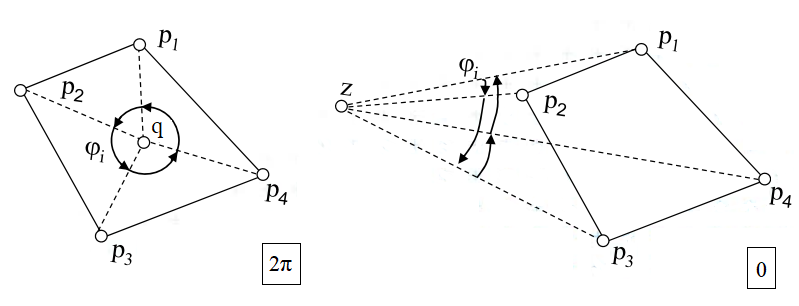
\includegraphics[height=40mm]{images/winding_number.PNG}\]
\[\textit{\footnotesize{Obr. 4 - Winding Number algoritmus}}\\\]

Hlubší popis metody je v následujícím pseudokódu:\\
\vspace{0.2cm}\\
\indent\textit{{1.~}Zjisti počet vrcholů polygonu $n$}\\
\indent\textit{{2.~}Inicializuj součet úhlů mezi definovaným bodem a hranou polygonu na 0}\\
\indent\textit{{3.~}\textbf{Projdi} jednotlivé vrcholy $p_{i}$ polygonu:}\\
\indent\indent\textit{{4.~}Zjisti polohu bodu $q$ vůči přímce $qp_{i}$}\\
\indent\indent\textit{{5.~}Vypočti úhel mezi přímkami $qp_{i}$, $qp_{i+1}$}\\
\indent\indent\textit{{6.~}\textbf{Když} je bod v levé polorovině,}\\
\indent\indent\indent\textit{{7.~}Přičti úhel k celkovému součtu uhlů}\\
\indent\indent\textit{{8.~}\textbf{Když} je bod v pravé polorovině,}\\
\indent\indent\indent\textit{{9.~}Odečti úhel od celkového součtu úhlů}\\
\indent\indent\textit{{10.~}\textbf{Jinak,}}\\
\indent\indent\indent\textit{{11.~}Leží-li bod $q$ mezi body $p_{i}$ a $p_{i+1}$, bod se nachází na hraně a ukončí výpočet}\\
\indent\textit{{12.~}\textbf{Když} je celkový součet úhlů roven 2$\pi$:}\\
\indent\indent\textit{{13.~}Bod je uvnitř polygonu}\\
\indent\textit{{14.~}\textbf{Jinak} je vně polygonu.}\\
\vspace{0.2cm}\\
V rámci tohoto algoritmu může nastat situace, která je nutná v rámci algoritmu ošetřit:\begin{itemize}
    \item bod $q$ je totožný s vrcholem.
\end{itemize}
Zda bod $q$ je totožný s vrcholem zjistíme tak, že při výpočtu směrnice bude jedna ze složek nulová.
Při porovnání Point-in-location a Winding Number zjišťujeme, že při jednoduchém mnohoúhelníku (tj. nemá žádné vlastní průsečíky) obě metody dávají stejný výsledek pro všechny body. Ovšem pro nejednoduché polygony dávají tyto dvě metody různé výsledky. \textit{„Například, když se mnohoúhelník překrývá sám se sebou, zjistí se, že body v oblasti překrytí jsou vně pomocí crossing number, kde pro Winding Number je znázorněno jako uvnitř" (Kumar, Bangi 2018, s. 550).} V porovnání s algoritmem Ray Crossing, je algoritmus Winding Number 20 krát pomalejší. (Felkel 2016)
\section{\large{Data}}
Vstupem jsou polygonové vrstvy ve formátu \emph{.shp} a bod \emph{q}. První polygonová oblast byla náhodně vybraná oblast polygonů obcí a pravidelná síť polygonů. Výstupem je grafické znázornění polygonů, které obsahují analyzovaný bod \emph{q}. Bod \emph{q} je bodem vstupu, který je vybrán na základě uživatele.
\section{\large{Dokumentace}}
Program je rozdělen do tří modulů. Modul \emph{Mainform.py} je převážně vygenerován pomocí softwaru QT Creator a slouží k vytvoření uživatelského rozhraní. Modul \emph{Algorithm.py} obsahuje algoritmy pro analýzu vzájemné polohy bodu a polygonů. Modul \emph{Draw.py} slouží především pro propojení předešlých dvou modulů, k zajištění vizualizace vstupu a výstupu a k volbě algoritmu.
\subsection{\small{Modul Mainform.py}}
Tento modul obsahuje třídu \texttt{Ui\_Mainform}, která je vytvořena automaticky pomocí QT Creatoru (Obr. 5). Tato třída byla posléze doplněna o  tři metody, které se spustí při interakci s uživatelským rozhraním. Metoda \emph{SelectFile}, která při zmáčknutí stejnojmenného tlačítka, vyvolá dialogové okno, kde je možné zvolit formát \emph{shapefile} se vstupními daty. Dále načte aktuální velikost okna, do kterého budou data vykresleny a zavolá funkci z modulu \emph{Draw.py}. Po stisknutí tlačítka \emph{„Analyse"} se spustí stejnojmenná metoda, která rozhodne, který algoritmus pro analýzu polohy bodu a polygonu využije a následně jej spustí. Metoda \emph{Change Algorithm} se zavolá při zmáčknutí tlačítka \emph{„Change Algorithm“} a slouží k výběru a k vizualizaci aktuálně zvoleného algoritmu.\\
\[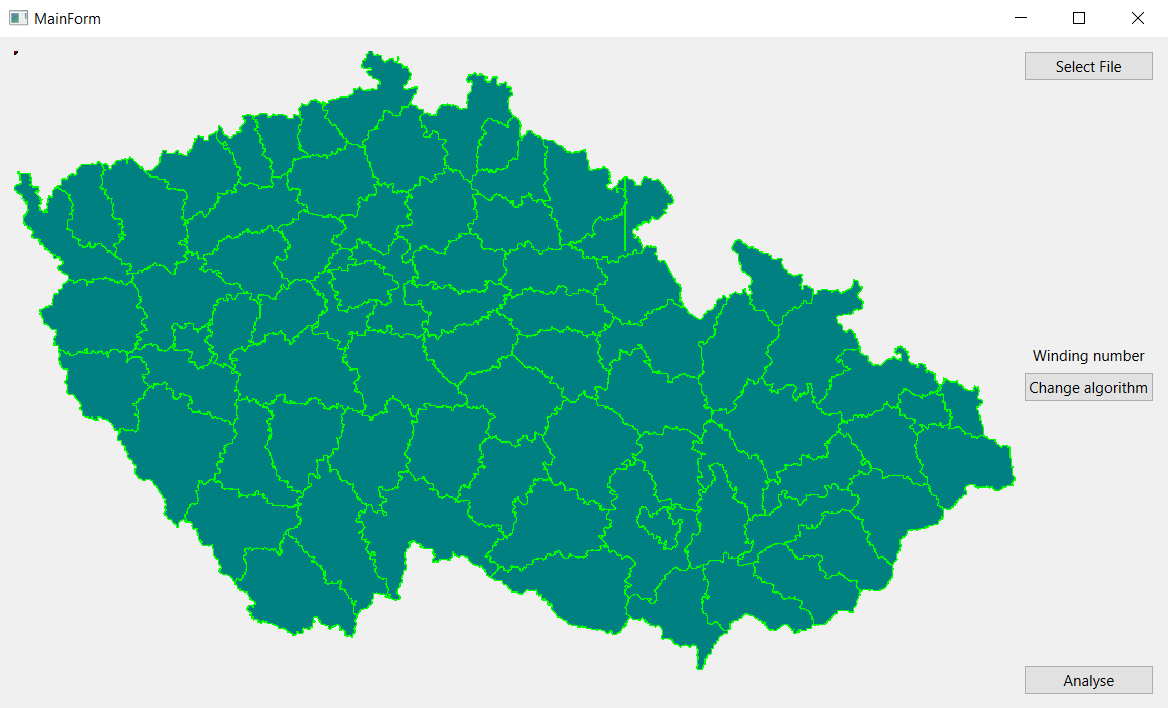
\includegraphics[height=85mm]{images/p_i_p.PNG}\]
\[\textit{\footnotesize{Obr. 5 - Náhled uživatelského rozhraní}}\\\]
\subsection{\small{Modul Draw.py}}
Tento modul obsahuje třídu \texttt{Draw}, kterou dědí od třídy \texttt{QWidget} z knihovny PyQt6. Na začátku se inicializuje proměnná \emph{q}, jako formát \emph{QPoint}. To umožňuje do \emph{q} ukládat souřadnice \emph{x} a \emph{y}. Do této proměnné se nahraje vstupní analyzovaný bod. Dále se inicializuje list \emph{polygons}, který ponese jednotlivé vstupní polygony. Další proměnná \emph{res} ve formátu \emph{list} bude zaručovat uchování výsledků a proměnná \emph{algorithm} nese informaci o aktuálně zvoleném výpočetním algoritmu.\\
První metoda v třídě \texttt{mousePressEvent} při stisknutí pravého tlačítka v uživatelském rozhraní v rozmezí vykreslovací plochy odečte aktuální souřadnice kurzoru \emph{x} a \emph{y} a uloží je pod \emph{q}. Následně zavolá metodu pro vykreslení. Metoda vykreslení \emph{paintEvent} definuje, jak se budou jednotlivé objekty třídy vykreslovat. Vykreslí všechny polygony v proměnné \emph{polygons}. U těchto polygonů je zvolena barva na základě výsledku, zda je hledaný bod uvnitř, či vně. Když výsledky ještě nejsou k dispozici (při prvním načtení polygonu), jsou všechny polygony stejné barvy. Dále jsou zde parametry pro vykreslení analyzovaného bodu.\\
V metodě \emph{loadPolygons} je nejprve načtena cesta ke vstupním datům. Když není zvolena žádná cesta, metoda se ukončí. Dále je načten vstupní shapefile. Data z tohoto shapefilu jsou převedeny do formátu \emph{QPolygon}. Následně tyto data musejí být ještě musejí být zobrazena do lokálního souřadnicového systému, který je definován velikostí okna. Takto transformovaná data jsou poté jako jednotlivé polygony vloženy do listu \emph{polygons}. Metoda \emph{switchAlgorithm} zajišťuje přepínání mezi algoritmy. Aktuální algoritmus ukládá do proměnné \emph{algorithm}. Poslední metody v této třídě jsou \emph{gettery}, které vracejí list vstupních polygonů a bod \emph{q}.
\subsection{\small{Modul Algorithm.py}}
Tento modul obsahuje dvě třídy. Každá z nich představuje jeden z výpočetních algoritmů - Winding Number nebo Ray Crossing. Třída \texttt{Winding\_num} tedy obsahuje metody k analýze vzájemné polohy bodu a polygonů pomocí metody Winding Number. První metoda této třídy - \emph{getPointAndLinePosition} - zjišťuje, jestli se daný bod \emph{q} nachází v pravé či levé polorovině od přímky definované dvěma body $p_{1}$ a $p_{2}$. Když je v levé, metoda vrací 1, v pravé 0 a když je bod kolineární, vrací hodnotu -1. Metoda \emph{get2LinesAngle} má na vstupu 4 body, které definují 2 přímky, u nichž je zjišťován úhel, který spolu svírají.\\
Hlavní metoda této třídy - \emph{getPositionPointAndPolygon} - zjišťuje vzájemnou polohu daného bodu a polygonu. Metoda vrací 1 pro bod uvnitř polygonu, nebo pro bod na hraně a ve vrcholu. Pro bod vně polygonu vrací 0.
Druhá třída  - \texttt{Ray\_cross} - využívá k analýze algoritmus Ray Crossing. První metoda - \emph{setLocalCoordinates} - převede souřadnice vrcholu polygonu tak, aby jejich počátek byl v analyzovaném bodu \emph{q}. Vrátí vrchol v lokálních souřadnicích s počátkem v bodu \emph{q}.\\
Metody \emph{getCrossingStatusU} a \emph{getCrossingStatusL} jsou si velice podobné. Obě metody analyzují, zda úsečka definovaná body $p_{i}$ a $p_{i-1}$ protíná osu y z pohledu z horní poloroviny a dolní poloroviny. Metody vracejí hodnotu \emph{True}, když dochází ke křížení a \emph{False}, když nikoli.\\
Hlavní metoda této třídy se opět nazývá \emph{getPositionPointAndPolygon} a zjišťuje vzájemnou polohu daného bodu a polygonu, nyní však využívá postupu algoritmu Ray Crossing.
\clearpage
\newpage
\section{\large{Závěr}}
Program by měl umět pracovat se singularitami jako je bod na hraně nebo ve vrcholu polygonu. Program by bylo možné vylepšit a zrychlit tím, že při určení vztahu bod-polygon byl bod uvnitř, výpočet tím byl zastaven a následně výsledek vizualizován. Nyní vždy za každé situace program prohlíží všechny vstupní polygony. Dále by mohlo být rozšířeno uživatelské rozhraní o tlačítko \emph{Clear}. Do programu by ještě mohla být přidána funkce, kdy se při zvětšení okna polygony automaticky překreslí na danou velikost. Nyní se polygony vykreslí do velikosti okna odečtené při jejich nahrávání.
\clearpage
\newpage
\section{\large{Seznam literatury}}
FELKEL, P. (2016): Geometric Searching Part 1: Point Location. Computational Geometry. Praha, 45 s.\\
\vspace{0.1cm}\\
KUMAR, G. N., BANGI, M. (2018): An Extension to Winding Number and Point-in-Polygon Algorithm. IFAC, vol. 51, s. 548-553.\\
\vspace{0.1cm}\\
O'ROURKE, J. (1998): Computational Geometry in C. Second Edition. Cambridge University Press, 392 s.\\
\vspace{0.1cm}\\
ŽÁRA, J., BENEŠ, B., SOCHOR, J., FELKEL, P. (2004): Moderní počítačová grafika. Computer Press, Brno, 609 s.\\
\end{document}